\chapter{Hall measurements on \acs{BSCO}}
    \label{Sec:HallBSCO}

\begin{chapterabstract}
Low (\unit{1.5}{\kelvin}) to high (\unit{300}{\kelvin}) temperature Hall measurements are presented on \ac{BSCO} over a wide doping range spanning the slightly underdoped to the far overdoped. The Hall and resistivity data is modeled using the Ong construction to determine the relative magnitudes of the scattering terms. In addition a novel doping assignment scheme based on new \ac{TL2201} \ac{dHvA} results is trialled and was found to give slightly higher dopings than the Ando method which compares room temperature Hall data to \ac{LSCO} and the Presland/Tallon method which scales normalised $T_c$ values to a `universal' parabola.
\end{chapterabstract}


\section{Sample growth}

The samples were grown by Prof. Takeuchi's group in Sendai University, Japan in May 2009 using the floating zone technique. Here powders of the correct stoichiometry are compacted into a rod and fed slowly through a furnace. A region towards the centre of the furnace heats the powders into a viscous melt, just below this region is a seed crystal. As the end of the rod passes through the melt region, it meets the seed crystal below and solidifies epitaxially onto it. The impurities are held in the melt portion of the crystal by a thermodynamic energy gradient. The rod continues to be slowly passed through the melt region, continually solidifying into the single crystal below until the entire rod has passed through and the growth is over. The end portion, containing the impurities is then removed. Samples from the same growth batch have previously been studied using \ac{ARPES} and \ac{STM} by members of the Sendai group~\cite{Wise2009, Wise2008, Kondo2007, Kondo2005, Kondo2010, Kondo2009, Kondo2006, Kondo2007}.

Table~\ref{Tab:ResH:SampleGrowthDetails} lists the nominal stoichiometries of the samples grown as well as the annealing conditions. Also listed are the \emph{nominal} $T_c$ values for the source crystals which are used to name the samples, the actual measured $T_c$ values of individual samples for the purposes of doping determination are slightly different due to different definitions of $T_c$\footnote{The source crystals were defined based on the zero value $T_c$, the $T_c$ for doping purposes is defined as the mid-point of the transition with an error based on the difference between the mid-point and the zero-point.}.
% \begin{table}
%     \begin{center}
%            \caption{Doping as determined by the Tallon relation, the Ando relation and scaling to \ac{TL2201} data as described in the method section.}
%         \begin{tabular}[htbp]{lrrrr}
% \toprule
% Sample	& $T_c$ ($K$)   & $p_{\textrm{Tallon}}$	& $p_{\textrm{Ando}}$	& $p_{\textrm{Tl}}$	\\
% \midrule
% B00KOD1A	& $0.0\pm1.0$	& $0.270\pm0.003$	& $0.223\pm0.002$	& $0.311\pm0.004$	\\
% B07KOD2		& $11\pm3.8$	& $0.252\pm0.013$	& $0.212\pm0.008$	& $0.271\pm0.013$	\\
% B16KOD1A	& $17\pm1.0$	& $0.240\pm0.004$	& $0.206\pm0.002$	& $0.249\pm0.004$	\\
% B30KOD3		& $29\pm0.5$	& $0.209\pm0.003$	& $0.188\pm0.002$	& $0.209\pm0.003$	\\
% B32KOP1		& $36\pm1.0$	& $0.160\pm0.018$	& $0.160\pm0.010$	& $0.160\pm0.018$	\\
% B32KOP4		& $35\pm2.0$	& $0.178\pm0.026$	& $0.170\pm0.015$	& $0.178\pm0.026$	\\
% B30KUD3		& $32\pm1.0$	& $0.123\pm0.008$	& $0.139\pm0.005$	& $0.123\pm0.008$	\\
% B28KUD3A	& $31.5\pm1.0$	& $0.121\pm0.008$	& $0.138\pm0.004$	& $0.121\pm0.008$	\\
% \bottomrule
%         \label{Tab:ResH:Dopings}
%         \end{tabular}
%     \end{center}
% \end{table}

\begin{table}
    \begin{center}
           \caption{Growth details for the \ac{BSCO} samples. OD, OP and UD stand for over, optimally and under doped respectively. $T_c$ values are nominal.}
        {\small \begin{tabular}[htbp]{lllllllll}
\toprule
\multicolumn{6}{c}{Nominal composition} & & & \\
Bi  & Pb  & Sr  & La  & Cu  & O   & $T_c$   & Reg.  & Annealing conditions \\
\midrule
1.72    & 0.38  & 1.85  & 0.0   & 1.0   & 6+d   & $<$2  & OD    & \unit{400}{\celsius}, \unit{96}{\hour} in \unit{2.5}{\textrm{atm.}} O$_2$ \\
1.72    & 0.38  & 1.85  & 0.0   & 1.0   & 6+d   & 7     & OD    & \unit{750}{\celsius}, \unit{24}{\hour} in air \\
1.72    & 0.38  & 1.85  & 0.0   & 1.0   & 6+d   & 16    & OD    & \unit{550}{\celsius}, \unit{72}{\hour} in flowing N$_2$ \\
1.35    & 0.85  & 1.47  & 0.38  & 1.0   & 6+d   & 30    & OD    & As grown \\
1.35    & 0.85  & 1.47  & 0.38  & 1.0   & 6+d   & 32    & OP    & \unit{650}{\celsius}, \unit{72}{\hour} in flowing N$_2$ \\
1.2     & 0.90  & 1.30  & 0.55  & 1.0   & 6+d   & 30    & UD    & As grown \\
1.2     & 0.90  & 1.30  & 0.55  & 1.0   & 6+d   & 28    & UD    & \unit{650}{\celsius}, \unit{72}{\hour} in flowing N$_2$ \\
\bottomrule
        \label{Tab:ResH:SampleGrowthDetails}
        \end{tabular}}
    \end{center}
\end{table}

\pagebreak
The samples are named according the convention,
\begin{quote}
\code{B<Tc>K<UD/OP/OD><Crystal No.><Sample No.>}
\end{quote}
where UD/OP/OD stands for underdoped, optimally doped and overdoped respectively. So for example `B00KOD2A' refers to the sample `A' taken from the crystal `B00KOD2' --- the second overdoped crystal with a nominal $T_c$ of $\unit{0}{K}$.

\section{Size determination}

Thicknesses were determined for some of the samples using the \ac{FIB} or the optical microscope as described in the methods section. These measurements were performed with the help of Dr. P. Heard. The thicknesses used to calculate absolute values of $R_H$ are listed in table~\ref{Tab:ResH:Thicknesses} and are marked in grey. \ac{FIB} results are given for areas as close to the two voltage contacts that were visible in the scans. As can be seen in the example scan shown in figure~\ref{Fig:ResH:FIBExamples}, there is some variation in the depth along the sample length.
\begin{figure}[htbp]
	\begin{center}
		\includegraphics[scale=0.9]{Chapter-HallBSCO/Figures/FIBExamples/FIBExamples}
		\caption{Top shows an image composited from several \ac{FIB} scans along the length of sample B00KOD1A, with bottom right showing a detail of the right voltage leg. Bottom left shows an oblique top down view of sample B30KOD3.}
		\label{Fig:ResH:FIBExamples}
	\end{center}
\end{figure}

The two scans shown are of good quality, however for the purpose of estimating errors in the thickness some of the scans presented problems. Samples B26KOD1A, B28KUD3A, B30KOD2 and B30KUD3 were obscured with the grease applied as part of the pulsed field measurements. Other samples were not correctly earthed such as B28KUD3B which made the images dark, whilst samples B07KOD2 and B32KOP3 were very flaky under close scrutiny. A scan of B30KOD3 showed that it was partially split in the ab plane which may contribute to systematic error in thickness estimate. In all these cases, the estimate in the thickness error was adjusted accordingly to compensate. A more comprehensive set of \ac{FIB} scans, including images of the split in the layers can be found in Appendix~\ref{Appendix:FIBScans}.

The oblique view of B30KOD3 in figure~\ref{Fig:ResH:FIBExamples} shows a clear misalignment of the voltage legs to the right of the image. This illustrates why it is necessary to take both positive and negative field sweeps in order to separate the magnetoresistance from the Hall components. This also explains why the length and width determinations were subject to large errors which affects the absolute value of the in-plane resistivity calculations.

\begin{table}
    \begin{center}
           \caption{Sample measurements as determined by optical microscope measurements and thickness as determined by \ac{FIB}. Samples highlighted in grey were used for determining absolute values of $R_H$. A and B refer to each of the two contacts visible to the \acs{FIB} scan.}
        {\small \begin{tabular}[htbp]{lrrrrr}
\toprule
	& \multicolumn{3}{c}{Optical}			& \multicolumn{2}{c}{\acs{FIB}}		\\
Sample  & Length (\unit{\micro\metre})	& Width (\unit{\micro\metre})		& Thick. (\unit{\micro\metre})	& Contact A (\unit{\micro\metre})    & Contact B (\unit{\micro\metre})    		\\

\midrule
\cellcolor[gray]{0.9}B00KOD1A	& \cellcolor[gray]{0.9}$781\pm123$	& \cellcolor[gray]{0.9}$157\pm49$	& \cellcolor[gray]{0.9}N/A		& \cellcolor[gray]{0.9}$45\pm1$	& \cellcolor[gray]{0.9}$50\pm5$	\\
B00KOD1B	& $627\pm49$	& $196\pm44$	& $39\pm5$ 	& $43\pm1.5$	& $45\pm1.5$	\\
B07KOD1		& $1277\pm74$	& $392\pm49$	& $29\pm10$	& N/A		& N/A		\\
\cellcolor[gray]{0.9}B07KOD2		& \cellcolor[gray]{0.9}$1061\pm69$	& \cellcolor[gray]{0.9}$333\pm74$	& \cellcolor[gray]{0.9}N/A		& \cellcolor[gray]{0.9}$20\pm5$ 	& \cellcolor[gray]{0.9}$30\pm1$ 	\\
\cellcolor[gray]{0.9}B16KOD1A	& \cellcolor[gray]{0.9}$795\pm34$	& \cellcolor[gray]{0.9}$299\pm34$	& \cellcolor[gray]{0.9}N/A		& \cellcolor[gray]{0.9}$24\pm1$ 	& \cellcolor[gray]{0.9}$24\pm1$ 	\\
B16KOD2A	& $358\pm29$	& $172\pm54$	& $9\pm1$ 	& N/A		& N/A		\\
B16KOD3		& $1122\pm44$	& $368\pm83$	& N/A		& $25\pm2$ 	& $24\pm2$ 	\\
B30KOD1	 	& $436\pm34$	& $250\pm44$	& $21\pm2$ 	& N/A		& N/A		\\
B30KOD2		& $344\pm44$	& $137\pm29$	& $20\pm5$ 	& $15\pm4$	& $15\pm4$	\\
\cellcolor[gray]{0.9}B30KOD3 	& \cellcolor[gray]{0.9}$255\pm49$	& \cellcolor[gray]{0.9}$98\pm25$ 	& \cellcolor[gray]{0.9}N/A		& \cellcolor[gray]{0.9}$16.5\pm1.5$	& \cellcolor[gray]{0.9}$19\pm1$	\\
\cellcolor[gray]{0.9}B32KOP1 	& \cellcolor[gray]{0.9}$658\pm83$	& \cellcolor[gray]{0.9}$397\pm34$	& \cellcolor[gray]{0.9}N/A		& \cellcolor[gray]{0.9}$6.5\pm1.5$	& \cellcolor[gray]{0.9}$6.5\pm1.5$	\\
B32KOP2		& $441\pm25$	& $226\pm20$	& $10\pm1$ 	& N/A		& N/A		\\
B32KOP3		& $437\pm34$	& $118\pm20$	& N/A		& $6\pm1$ 	& $6\pm1$ 	\\
B32KOP4 	& $427\pm74$	& $137\pm39$	& N/A		& $9\pm3$ 	& $9\pm3$ 	\\
B30KUD1A	& $622\pm49$	& $447\pm25$	& $36\pm3$ 	& N/A		& N/A		\\
B30KUD1B	& $828\pm34$	& $471\pm64$	& $35\pm3$ 	& N/A		& N/A		\\
B30KUD2 	& $545\pm69$	& $152\pm39$	& N/A		& $5 \pm1$ 	& $5 \pm1$ 	\\
\cellcolor[gray]{0.9}B30KUD3 	& \cellcolor[gray]{0.9}$476\pm49$	& \cellcolor[gray]{0.9}$118\pm34$	& \cellcolor[gray]{0.9}N/A		& \cellcolor[gray]{0.9}$7\pm2$ 	& \cellcolor[gray]{0.9}$7\pm2$ 	\\
B28KUD2A	& $657\pm29$	& $250\pm39$	& $11\pm1$ 	& N/A		& N/A		\\
\cellcolor[gray]{0.9}B28KUD3A	& \cellcolor[gray]{0.9}$633\pm49$	& \cellcolor[gray]{0.9}$142\pm34$	& \cellcolor[gray]{0.9}N/A		& \cellcolor[gray]{0.9}$16\pm3$	& \cellcolor[gray]{0.9}$16\pm3$	\\
B28KUD3B	& $653\pm44$	& $216\pm49$	& N/A		& $16\pm3$	& $16\pm3$	\\
\bottomrule
        \label{Tab:ResH:Thicknesses}
        \end{tabular} }
    \end{center}
\end{table}



\section{Temperature sweeps}

Figure~\ref{Fig:ResH:TSweeps} shows the in-plane resistivity, $\rho(T)$ for each of the samples in zero field taken in the \ac{VTI} in the Polo magnet. From this plot we can characterise the \Tc of the samples and find the residual resistivity, $\rho_0$ by using simple linear fits to the data above the transition temperatures and extrapolate back to zero. Table~\ref{Table:ResH:TSweepFitsParams} show the fit parameters for each of the samples. 
\begin{table}
	\begin{center}
       	\caption{Fits parameters to $\rho = \rho_0 + \rho_1T$ for zero field resistivity data above $T_c$ as well as $T_c$ values determined from the same plots. Fits at low $T$ are shown in inset to figure~\ref{Fig:ResH:TSweeps}.}
		{\small \begin{tabular}[htbp]{lrrrr}
\toprule
Sample		& $\rho_0 (\unit{\micro\ohm\centi\metre})$	& $\rho_1 (\unit{\micro\ohm\centi\metre})$  & $T_c$ (\unit{\kelvin})	& $T_c/T_c(\textrm{max})$	\\
\midrule
B00KOD1A	& 40.7		& 0.454     & $0\pm1.0$	    & $0.00\pm0.03$	\\
B07KOD2		& 73.0		& 1.026     & $11\pm3.8$	& $0.31\pm0.11$	\\
B16KOD1A	& 49.9		& 0.843     & $17\pm1.0$	& $0.47\pm0.03$	\\
B30KOD3		& 15.9		& 0.578     & $29\pm0.5$	& $0.81\pm0.01$	\\
B32KOP1		& 54.2		& 0.824     & $36\pm1.0$	& $1.00\pm0.03$	\\
B32KOP4		& 55.6		& 1.904     & $35\pm2.0$	& $0.97\pm0.06$	\\
B30KUD3		& 123.0		& 2.233     & $32\pm1.0$	& $0.89\pm0.03$ \\
B28KUD3A	& 22.6		& 0.806     & $32\pm1.0$	& $0.89\pm0.03$	\\
\bottomrule
		\label{Table:ResH:TSweepFitsParams}
		\end{tabular} }
	\end{center}
\end{table}
The residual resistivities are very good with only one being above \unit{100}{\micro\ohm\centi\metre} and most below \unit{70}{\micro\ohm\centi\metre} which has been cited as being exceptionally good for \ac{BSCO}~\cite{Ando1999}. Moreover the \Tc of the optimally doped sample is \unit{36}{\kelvin} which is amongst the highest reported~\cite{Ando1999} which again is testament to the crystal quality. $\rho_0$ generally increases as you move away from critical doping which lends support to the notion of the La doping increasing the disorder in the CuO layers.

The inset to figure~\ref{Fig:ResH:TSweeps} shows the $\rho(\unit{300}{\kelvin})$ values for the samples along with error bars due to uncertainty in the size determination. As we saw in the previous section, there is significant misalignment and overall width to the voltage contacts which lead to large systematic errors which affect scaling only. Nonetheless, there appears to be an downward trend in resistivity as doping is increased. The circled points are B30KUD3 in both the overdoped and underdoped position and although the position is perhaps more fitting in the underdoped position, there error bars leave the overdoped point well within the overall trend.


% \begin{table}
% 	\begin{center}
%        	\caption{Fits parameters to $\rho = \rho_0 + \alpha_1T +
%        	\alpha_2T^2$ for zero field resistivity data above $T_c$.
%        	Fits at low $T$ are shown in inset to figure~\ref{Fig:ResH:TSweeps}}
% 		\begin{tabular}[htbp]{lrrr}
% \toprule
% Sample		& $\rho_0 (\times10^-2)$	& $\alpha_1 (\times10^{-4})$	& $\alpha_2 (\times10^{-7})$	\\
% \midrule
% B00KOD1A	& 12.26		& 6.895		& 14.394		\\
% B07KOD2		& 9.03		& 7.740		& 8.459			\\
% B16KOD1a	& 4.25		& 4.809		& 3.610			\\
% B30KOD3		& 1.43		& 3.385		& 4.595			\\
% B32KOP1		& 1.20		& 2.596		& -0.810		\\
% B32KOP4		& 2.76		& 21.886	& -8.862		\\
% B30KUD3		& 18.80		& 38.028	& -4.385		\\
% B28KUD3a	& 2.71		& 18.447	& -6.756		\\
% \bottomrule
% 		\label{Table:ResH:TSweepFitsParams}
% 		\end{tabular}
% 	\end{center}
% \end{table}


\section{Hall plots}

Figures~\ref{Fig:ResH:HallIndividualOD}, \ref{Fig:ResH:HallIndividualOP} and \ref{Fig:ResH:HallIndividualUD} show the Hall coefficients extracted as described in the methods section for samples progressing from overdoped, optimally doped to underdoped respectively. Where appropriate, the data is compared to that from Ando \etal~\cite{Ando1999}. Red lines in the plots are guides to the eye.

For the samples of $T_C >= \unit{28}{\kelvin}$ there are some data which did not reach sufficient field to obtain linear behaviour which are circled with a dashed line in the plots. For sample B30KOD2, many of the sweeps for $T < \unit{45}{\celsius}$ showed significant hysteresis due to temperature drift. Despite temperature correction, many of the fits did not pass through the origin (circled in the figure) which is a good indicator that the true field suppressed linear Hall has not been obtained. The same goes for the circled points on the B30KUD2 plot and another data point at $T=\unit{1.5}{\kelvin}$ and $R_H = \unit{$7.3\times10^{-3}$}{\centi\metre\cubed}$ from the first trip to \ac{LNCMI} which is outside the plot boundary as well as data points on the plot for B28KUD3B. The data sets are combined, minus the points highlighted in the previous paragraph, in the main panels of figure~\ref{Fig:ResH:InvHallCombined} alongside the data from the Ando paper.

\begin{figure}[htbp]
	\begin{center}
		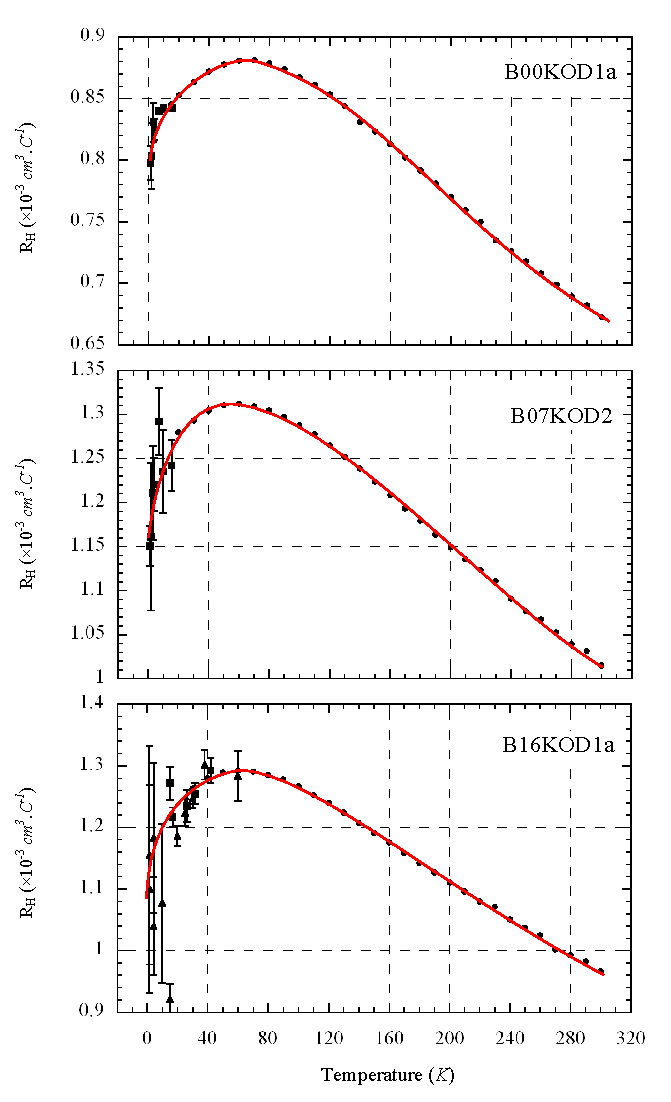
\includegraphics[scale=0.9]{Chapter-HallBSCO/Figures/HallIndividual/HallIndividualOD}
		\caption{$R_H$ for underdoped samples of \ac{BSCO}. Plots show results from, $\bullet$ Polo in June 2010, $\blacktriangle$ \ac{LNCMI} in June 2009, $\blacktriangledown$ \ac{LNCMI} in Feb 2010, $\blacksquare$ Nijmegen in May 2010. Symbols for comparable samples are marked on the plots. Red lines are a guide to the eye.}
		\label{Fig:ResH:HallIndividualOD}
	\end{center}
\end{figure}

\begin{figure}[htbp]
	\begin{center}
		\includegraphics[scale=0.9]{Chapter-HallBSCO/Figures/HallIndividual/HallIndividualOP}
		\caption{$R_H$ for underdoped samples of \ac{BSCO}. Plots show results from, $\bullet$ Polo in June 2010, $\blacktriangle$ \ac{LNCMI} in June 2009, $\blacktriangledown$ \ac{LNCMI} in Feb 2010, $\blacksquare$ Nijmegen in May 2010. Symbols for comparable samples are marked on the plots. Dashed lines indicate points where the field was not sufficient to achieve linear behaviour. Red lines are a guide to the eye.}
		\label{Fig:ResH:HallIndividualOP}
	\end{center}
\end{figure}

\begin{figure}[htbp]
	\begin{center}
		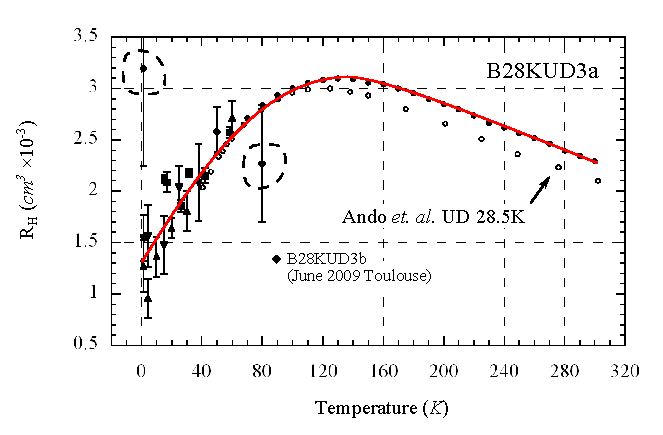
\includegraphics[scale=0.9]{Chapter-HallBSCO/Figures/HallIndividual/HallIndividualUD}
		\caption{$R_H$ for underdoped samples of \ac{BSCO}. Plots show results from, $\bullet$ Polo in June 2010, $\blacktriangle$ \ac{LNCMI} in June 2009, $\blacktriangledown$ \ac{LNCMI} in Feb 2010, $\blacksquare$ Nijmegen in May 2010. Symbols for comparable samples are marked on the plots. Dashed lines indicate points where the field was not sufficient to achieve linear behaviour. Red lines are a guide to the eye.}
		\label{Fig:ResH:HallIndividualUD}
	\end{center}
\end{figure}
\begin{figure}[htbp]
	\begin{center}
		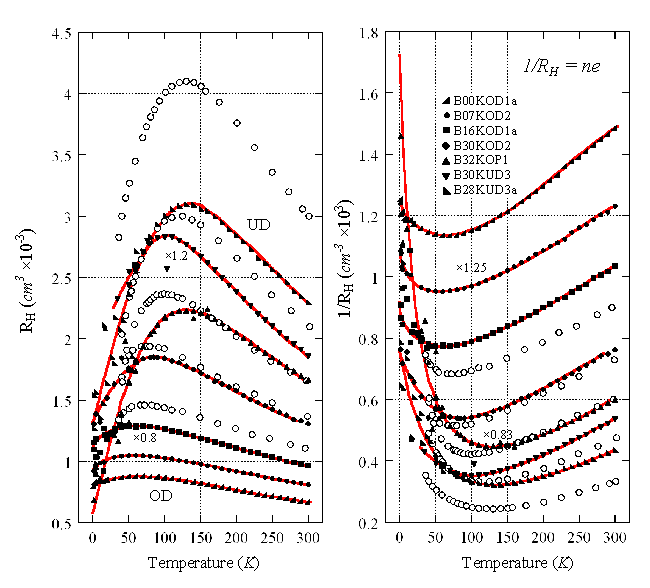
\includegraphics[scale=1.1]{Chapter-HallBSCO/Figures/InvHallCombined/InvHallCombined}
		\caption{Hall data in context with data from Ando \etal\cite{Ando1999} (open circles) which are in order of increasing $R_H$, 24KOD, 30KOD, 33KOP, 28.5KUD, 20KUD. Right panel shows the inverse hall data which relates to carrier density. Red lines are the same guides to the eye used in previous figures. Inset shows $R_H$ at \unit{300}{\kelvin} plus systematic error bars due primarily to uncertainty in thickness vs. doping scaled to \ac{TL2201} data. B30KUD3 (circled) is plotted in both the overdoped and underdoped positions.}
		\label{Fig:ResH:InvHallCombined}
	\end{center}
\end{figure}

With reference to figure~\ref{Fig:ResH:InvHallCombined} and in particular the new low temperature data points, we see that doping strongly affects the qualitative shape of the $R_H$ curves. Whilst the trend appears to be that $R_H(\unit{300}{\kelvin})$ decreases as doping increases as to be expected, the $R_H(\unit{0}{\kelvin})$ values all tend toward approximately similar values of around \unit{$0.5\times 10^{-3}$}{\centi\metre\cubed}to \unit{$1.5\times 10^{-3}$}{\centi\metre\cubed}. The most pronounced difference between high and low temperature values though is with the optimally doped samples which are around $\times 2.75$ greater at high temperature. Right down to \unit{0}{\kelvin} there is no sign change in $R_H$, which suggests that the hole pockets have higher mobility than the electron pockets across the range of dopings studied.

The error bars on the data points do not include error from the thicknesses which are systematic across the data points. The inset of figure~\ref{Fig:ResH:InvHallCombined} shows the $R_H$ values at \unit{300}{\kelvin} vs. doping for each of the samples with these error bars applied. The overall trend is downward with doping with the progression being approximately monotonic, however the exception is B16KOD1A which has a slightly lower $R_H$ than would be expected from a linear trend.

The Hall angle is plotted for each of the samples where $B=\unit{0}{\tesla}$ in-plane resistivity data is available in figure~\ref{Fig:ResH:HallAngle} with temperature raised to a fitted exponent, $\alpha$. In the original Chien analysis, $\alpha = 2$ but is allowed to vary here to observe deviations from the expected $T^2$ behaviour. Similar analysis was performed for resistivity data taken at $B=\unit{13}{\kelvin}$ and although these plots are not shown, the fitted $\alpha$ values are plotted in the bottom left subplot along with the $B=\unit{0}{\tesla}$ values. A nominal unitary field was used when calculating $\cot\theta_H$ and only data above the superconducting transition was fitted and is shown in the plots. Note that for the $B=\unit{13}{\tesla}$ case, the Hall data for the optimally doped sample B32KOP1 was compared with resistivity data for sample B32KOP4 which explains the slightly different doping value assigned to it. In this particular instance, it appears that the assignment of the sample B30KUD3 would be more suited to underdoped rather than overdoped.

\begin{figure}[htbp]
    \begin{center}
        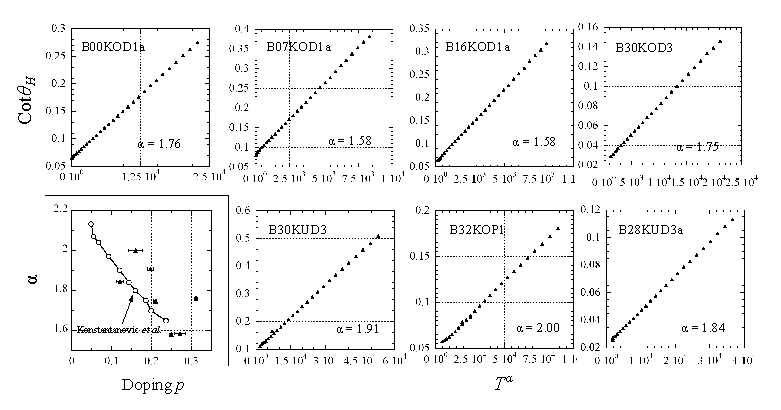
\includegraphics[scale=1.0]{Chapter-HallBSCO/Figures/HallAngle/HallAngle}
        \caption{Hall angle calculated with a nominal field of unity from resistivity data taken in zero field. Plot in bottom left shows the fitted exponent, $\alpha$, vs. doping compared with similar data on \ac{BSCO} from Konstantanovi\'c \etal~\cite{Konstantinovic2000} for both zero field resistivity data and resistivity data taken at \unit{13}{\kelvin} ($\cot\theta_H$ plots for $B=\unit{13}{\tesla}$ not shown)}
        \label{Fig:ResH:HallAngle}
    \end{center}
\end{figure}
With reference to the plot in the lower left, the fitted exponents approximately follow the same downward trend with doping as in \ac{BSCO} data from Konstantanovi\'c \etal~\cite{Konstantinovic2000} up to around $p=0.27$. In particular the $B=\unit{13}{\tesla}$ follows the curve reasonably closely before the upturn at $p=0.31$. Downward deviation from the $T^2$ behaviour at high temperatures (as indicated from a drop in the $\alpha$ exponent) at this point in the phase diagram has been previously interpreted to be due to the saddle point in the \ac{DOS} which is approaching from below the Fermi energy~\cite{Ando2004} which would also explain why there is a recovery toward $T^2$ behaviour between $p=0.27$ and $p=0.31$ as the flat portion of the \ac{DOS} passes above the Fermi energy. This would suggest that the van-Hove singularity peaks in the \ac{BSCO} phase diagram at around $p=0.25$, approximately where the B16KOD1A sample lies and where the room temperature $R_H$ value was also found to be slightly lower than expected. However this occurs at a higher doping than the Hashimoto paper would suggest~\cite{Hashimoto2008} (see figure~\ref{Fig:Intro:VanHoveBSCOLSCO}) and given the proximity of the van-Hove singularity, the low Hall coefficient should not be interpreted a simple indicator of carrier density. 
\begin{figure}[htbp]
    \begin{center}
        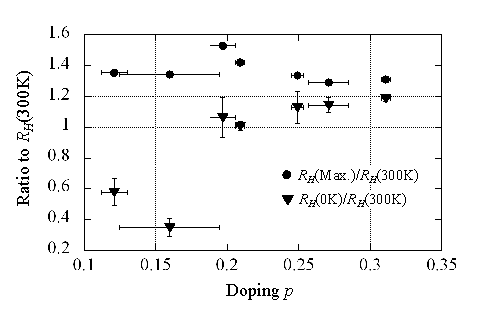
\includegraphics[scale=0.8]{Chapter-HallBSCO/Figures/RhRatios/RhRatios}
        \caption{Left shows ratio of $R_H$ values at the maximum of the Hall curves and at $T=\unit{0}{\kelvin}$ to the $T=\unit{300}{\kelvin}$ $R_H$ values. Errors in $R_H(\unit{0}{\kelvin}$ estimated from Hall plots, the value for B30KUD2 is estimated based on linear extrapolation. Right shows the temperature where the maximum $R_H$ occurs.}
        \label{Fig:ResH:RhRatios}
    \end{center}
\end{figure}

An alternate explanation based on the Narduzzo paper~\cite{Narduzzo2008} goes as follows. For $p \gtrsim 0.19$, $R_H(\unit{0}{\kelvin} > R_H(\unit{300}{\kelvin})$ as illustrated in figure~\ref{Fig:ResH:RhRatios}. If we assume there is not temperature dependent change of the Fermi surface such that would affect $\vect{v_F}$, then this can be explained by an temperature dependent increase in the anisotropy of the scattering. As detailed in the introduction, such scattering is thought to originate in the overdoped side of the phase diagram and is seemingly closely tied to superconductivity. The Narduzzo paper explores this possibility but ultimately could not definitively conclude that the scattering rate is proportional to $\cos^2(2\phi)$ as is the case in the Abdel-Jawad paper~\cite{Abdel-Jawad2007}.

When we consider the ratio of the maximum $R_H$ to the \unit{300}{\kelvin} value also plotted in figure~\ref{Fig:ResH:RhRatios} then we see that these values do not vary much at all with doping indicating that the scattering process that suppresses the low temperature Hall values only becomes dominant below the temperature where $R_H(\textrm{max})$ occurs. Moreover we note that the low temperature behaviour of $R_H$ which, although not possible to ascertain for certain due to the scatter in points, appears linear in temperature below $R_H(\textrm{max})$, which suggests that the same process explored above is $T$-linear in behaviour. Finally the temperatures of the maximums in $R_H$ are plotted in figure~\ref{Fig:ResH:RhRatios} and show a similar doping behaviour to the $\alpha$ fitted exponents.




% There seems to be little evidence of the transition of the doping from $p$ to $1+p$ which agrees with the notion that these dopings lie beyond where the change in the size of the Fermi surface is thought to take place~\cite{LeBoeuf2007}. 

%Divergence in resistivity occurs beyond UD 0K\cite{Ando2000}, well
%below our lowest nominal doping of ...

% Residual resistivity of ~20\mu\Ohm cm at optimal doping is very small
% and increases with La doping i.e. as become more underdoped
% \cite{Ando2000}





\section{Doping determination}
    \label{Sec:ResH:DopingDetermination}

As described in section~\ref{Sec:Intro:DeterminingDoping}, we compared the Hall values of our samples at high temperature to determine the doping similar to the method used by Ando \etal\cite{Ando2000}. In order to compare this method with other doping characterisation methods, the actual (i.e. not nominal) $T_c$ values for the samples were used from the resistivity curves shown in figure~\ref{Fig:ResH:TSweeps}. These values were input into the parabolic relation from Presland \etal~\cite{Presland1991} and Ando \etal~\cite{Ando2000}. This is then compared with the doping assignments which we make by matching $R_H(\unit{300}{\kelvin})$ in the \ac{BSCO} data from the previous section with that compiled in Kokalj \etal~\cite{Kokalj2012} on \ac{TL2201}. The results of these comparisons are shown in figure~\ref{Fig:ResH:DopingRh300}.
\begin{figure}[htbp]
    \begin{center}
        \includegraphics[scale=1.1]{Chapter-HallBSCO/Figures/DopingRh300/DopingRh300}
        \caption{Assigning the dopings of the \ac{BSCO} data such that $R_H(\unit{300}{\kelvin})$ values match those of \ac{TL2201}. Dashed line is a second order polynomial fit to the \ac{TL2201} data that is used to obatin the exact dopings.}
        \label{Fig:ResH:DopingRh300}
    \end{center}
\end{figure}
The \ac{TL2201} data does not span the entire range of $R_H(\unit{300}{\kelvin})$ values that the \ac{BSCO} covers, for this reason a second order polynomial is fit to the Kokalj data and the \ac{BSCO} doping is assigned to this curve. The underdoped sample B28KUD3a is far along the extrapolated curve, however still lies within the standard Presland/Tallon assignment as used to determine the dopings for the Konstantanovic data~\cite{Konstantinovic2001}.

Figure~\ref{Fig:ResH:Dopings} shows the dopings as determined by the three different methods outlined in the experimental methods chapter. The dopings of the crystals range from $p=0.12$ to $p=0.36$ hole per Cu atom with significant discrepancies between the methods. The Ando determination bunches the doping values around a much narrower range, whereas the dopings determined by comparing with the \ac{TL2201} \ac{dHvA} data, spread the overdoped values over a wider range. The Presland/Tallon method sits between the two. Most notable is that the dopings assigned by Kondo \etal~\cite{Kondo2004} from \ac{ARPES} measurements of the Fermi surface volume taken at \unit{200}{\kelvin}. These are for different samples from the same growth batch but show significantly higher still span of dopings between $p=0.25$ and $p=0.43$. It is not clear why there is a discrepancy given that both determinations are based measure of the Fermi surface in the normal state (the \ac{dHvA} begin field induced at low temperature and \ac{ARPES} being above $T_c$), however we believe that the \ac{ARPES} data may be subject to some kind of surface charge effect since it shows that the overdoped \unit{0}{\kelvin} sample has passed the van-Hove singularity when our Hall data (obtained from the sample bulk) does not show any evidence for this.

\begin{figure}[htbp]
    \begin{center}
        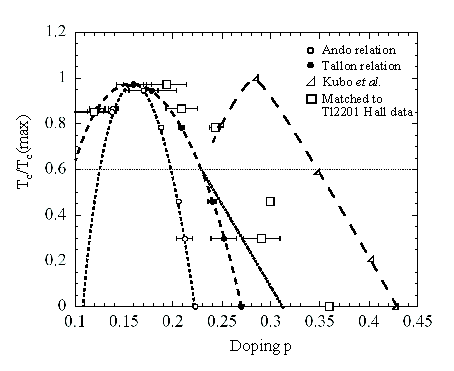
\includegraphics[scale=1.1]{Chapter-HallBSCO/Figures/Dopings/Dopings}
        \caption{Doping distributions for the three different methods. From left to right, B28KUD3A, B30KUD3 (Assume UD), B32KOP1, B32KOP4, B30KUD3 (Assume OD), B30KOD3, B16KOD1A, B07KOD2, B00KOD1A. Broken lines are a guide to the eye. Circled points are B30KUD3 for both the overdoped and underdoped scenarios.}
        \label{Fig:ResH:Dopings}
    \end{center}
\end{figure}

% \begin{figure}[htbp]
%     \begin{center}
%         \includegraphics[scale=1.2]{Chapter-HallBSCO/Figures/DRhoDtCurves/DRhoDtCurves}
%         \caption{$d\rho(T)/dT$ curves for each of the samples taken in \unit{0}{\tesla} and \unit{13}{\tesla} field. Note the evolution of the $T_{\textrm{coh}}$ gradient in the overdoped samples which give way to the $T^*$ kink in the underdoped samples, B30KUD3 has been repositioned to follow this trend.}
%         \label{Fig:ResH:DRhoDtCurves}
%     \end{center}
% \end{figure}
% The derivatives of the same resistivity curves in figure~\ref{Fig:ResH:TSweeps} are plotted in figure~\ref{Fig:ResH:DRhoDtCurves} along with derivatives to temperature sweeps taken at \unit{13}{\tesla}. Here we can see in the overdoped samples the distinct slope downwards towards \Tc which signifies the coherent quasiparticle region which begins at $T_{\textrm{coh}}$. This gradually levels out as doping is reduced until we observe a kink which marks the pseudogap temperature, $T^*$. The $T^*$ kink is weaker in B30KUD3 than the optimally doped samples and in fact only appears, at a much lower temperature, when the field is applied. This suggests that it is in fact more doped than the optimally doped samples rather than less doped as the nominal composition would suggest. If we consider B30KUD3 to be overdoped rather than underdoped then this trend continues right across the range of samples.


% Figure~\ref{Fig:ResH:Rh300Comparison} present Hall data at \unit{300}{\kelvin} again taken in the Polo with comparable data from Konstantinovi\'c \etal~\cite{Konstantinovic2001}.
% \begin{figure}[htbp]
%     \begin{center}
%         \includegraphics[scale=1.1]{Chapter-HallBSCO/Figures/Rh300Comparison/Rh300Comparison}
%         \caption{Hall data at \unit{300}{\kelvin} compared with similar data taken from refs.~\cite{Konstantinovic2001, Kokalj2012} using different doping assignments. From left: Tallon relation, Ando relation and scaling to \ac{TL2201} data. Red lines are guides to the eye, circled points are B30KUD3 in the overdoped and underdoped positions.}
%         \label{Fig:ResH:Rh300Comparison}
%     \end{center}
% \end{figure}
% It is clear that the Ando assignment of dopings is too confined with the data not at all following the respective curves whereas the Tallon relation follows much close the shape of the curve, although, perhaps this is not surprising given that the dopings in the Konstantinovo\'c paper were also assigned using the Tallon relation. However what is most interesting is that when compared with \ac{TL2201} data from Kokalj \etal~\cite{Kokalj2012} which we know is appropriate to scale to the \ac{TL2201} doping scheme, we see that of the three methods, scaling the \ac{BSCO} to the \ac{TL2201} \ac{dHvA} data matches the closest. On this rationale, we continue assuming that the \ac{TL2201} doping assignments are the correct ones.

% Also, referring to the circled points, we see that again the data is more consistent if we consider the B30KUD3 to be overdoped rather than underdoped. Looking back to the inset of figure~\ref{Fig:ResH:TSweeps} we see that there is large scatter in the data points due to uncertainty in the dimensions which were determined by optical microscope, however there is an approximate downward trend with doping which is similar to what is found in the literature~\cite{Ando2000, Ando1999, Konstantinovic2001, Ono2000}. Although B30KUD3 is more consistent to this trend in the underdoped position, the trend still lies with the error bars of the overdoped position. Looking ahead to the inset of figure~\ref{Fig:ResH:InvHallCombined} which shows $R_H$ values at \unit{300}{\kelvin} vs. doping, which depend only on the measurement of depth --- which was much more accurately determined by the \ac{FIB} --- we see that the underdoped position lies far outside the overall trend even when considering the error bars. 




\section{Conclusions}

High quality crystals of Pb and Sr doped \ac{BSCO} were sourced and studied in the normal state by high-field magnetotransport measurements down to low temperatures, thereby determining the low temperature Hall behaviour. The samples exhibited a sharp change in in the $R_H(\unit{0}{\kelvin})/R_H(\unit{300}{\kelvin})$ which coincides with various phenomena related to the pseudogap. This occurs in the field induced normal state which suggests that the scenario described in section~\ref{Sec:Intro:Pseudogap} where the pseudogap disappears at the top of the superconducting dome is not the correct one.

The data was modeled using a simple anisotropic model based on the Ong construction and was found to fit the relative scattering rates in the reasonably well it although consistently underestimated the residual resistivity term and for the overdoped samples overestimated the $T^2$ term. An increase in the $T$-linear term was observed to scale with doping similar to as found by Abdel-Jawad \etal~\cite{Abdel-Jawad2007}. This relatively crude model suggests that with further refinement it could be used to explain the physics at underdoped side of the phase diagram without resorting to complex Fermi surface reconstruction scenarios proposed by LeBeouf \etal The first port of call for the refinement would be the inclusion of the Fermi velocity in the scattering rate which may also improve the agreement in the overdoped side.

A novel doping determination technique is presented based on the method outlined by Ando \etal{} but comparing the \ac{BSCO} samples to the recently determined doping in overdoped \ac{TL2201} using \ac{dHvA}. The method assigns doping values that fall between the `universal' method of Presland/Tallon and those found from \ac{ARPES} measurements by Kondo \etal

A natural continuation of this work would include a more precise determination of the low field region to determine with more certainty if the low temperature behaviour is truly $T$-linear or it plateaus at very low temperatures as found by Balkirev \etal{} in underdoped samples~\cite{Balakirev2003} and then attempt to model it using the Ong construction.



